% Allow relative paths in included subfiles that are compiled separately
% See https://tex.stackexchange.com/questions/153312/
\providecommand{\main}{..}
\documentclass[\main/thesis.tex]{subfiles}
\externaldocument{}



\begin{document}

\chapter{Introduction}

 
\section{Our Goals and Findings}
Digital recordings of novel, one-shot\footnote{A single hit on the drum that captures its capabilities} drum sounds are not easy or cheap to find. New drum sounds can be obtained via live recordings of drums, layering existing drum sounds and often lengthy hacking of sound engineering techniques. The goal here is to create a new, virtual source of novel drum sounds, where most of the outputs are suitable substitutes for organic drums. In addition, given that a sound is percussive, we require the accurate categorization of drum-types.

We created systems capable of generating drum synthesizer programs, and measured the success rate by listening to the sound outputs. The survey of our best generative system showed that only 8\% of the sounds were deemed not percussive by both reviewers, and 30\% by at least one. With regards to agreement between manual and automatically assigned labels to drum sounds, our measurements showed Fleiss kappa scores of 0.3 or higher, indicating a moderate agreement~\footnote{These kappa scores nearly doubled when non-percussive sounds were removed from the survey}.


% These results indicate that the majority of sounds produced from our system are suitable substitutes for drum sounds. Among these percussive sounds, we found a moderate to high degree of agreement between the  automatically assigned drum labels and blinded, manual hearing tests.
% \subsection{Drums and Percussion}
% Drums are a subcategory of percussive instruments. Almost any object which is struck to produce noise can be referred to as a drum~\cite{latham2002oxford}. Under strict definitions, the terms can be used interchangeably~\cite{latham2002oxford}. We adapt this strict definition as our work is not concerned the delineation between the two overlapping concepts, but with creation of synthetic sounds which can be used by digital sound artists as replacements for organic drums or percussion. We often use the terms \enquote{drum} and \enquote{percussion} interchangeably.

\section{Why Does the World Need More Drums?}
Percussive sounds are often created by striking of a percussive instruments and used for creation of rhythm in compositions~\cite{needham1967percussion}. Kicks and snares are two of the most common examples of percussive sounds~\cite{barry2005drum}. We are looking for sounds which can be used as substitutes for drums in experimental and eclectic compositions and are not concerned with the nuances of drum vs percussive sounds. As a result, we often use \enquote{drum} and \enquote{percussion} interchangeably.

A common approach to creation of drum tracks for digital music is to combine short recordings of real-life drums and other percussive elements in order to create a virtual drum-kit. This approach frees artists from the need to obtain and store real life instruments while enabling endless combinatorial possibilities. However, by relying on recordings of \enquote{real life} drum sounds, we are limited by what instruments exist in the real world and whether or not we have access to clean, one-shot recordings. We believe that digital simulation of sound generation can alleviate these material limitations. 
 
\section{What Solution Do We Propose?}
We want to virtually create novel drum sounds. We need a generative source; One that produces audio based on some instructions. We also need a method of evaluation to help us determine which sounds resemble drums and are worth keeping. We also would like to know what instructions caused our audio source to make the sounds we liked, so we can modify and experiment with the instructions. In short, our approach requires virtual \textit{generation} and \textit{evaluation} of sounds. 

\section{What Tools Are at Our Disposal?}
\label{sec_tools_disposal}
We can conceptualize utilizing digital sound synthesis in various ways. An ideal scenario would be a graphical, 3D simulation of virtual drums where we can modulate parameters such as frame, skin and the type of impact before rendering the sound of the simulation. Unfortunately, such 3D systems are not yet practical \cite{langlois2016toward}. State of the art generative networks utilized in works by Ramires et al. \cite{ramires2020neural} and Aouameur et al.\cite{aouameur2019neural} 
are another promising avenue, but the computation costs and data requirements remain high. Here, we work towards tractable methods that utilize simple signal generation tools and machine learning techniques to rapidly generate new sounds and evaluate their desirability. Reduction of the examples necessary for effective learning is also a priority.
% Before we further cover details of the project, it's important to give a quick introduction to the basics of computerized audio generation and evaluation that were made use of in this project.
\subsection{How Can A Computer Make Sounds?}
\label{sec:computer_make_sound}
Most people can experience some\footnote{Human audible range is approximately 30Hz to 15000KHz} of the vibrations in their environments through sound. A computer can make a wide variety of audible vibrations in a number of ways: We can use it to record real life audio and play it back. We can hit it with drumsticks. We can also program it to make noise using software, usually by emulating the physical characteristics of basic waveforms by evaluating the output of periodic functions such as sines and cosines. Evaluation of basic periodic functions is the simplest form of software audio generation~\cite{mitchell2009basicsynthChap5}.

\enquote{Dialing tones} (DTMF) and emergency vehicle sirens are common examples of simple, digitally generated sounds. A simple method of making digital audio is feeding a range of equally spaced values between 0 and $2\pi$ to a sinusoidal function at a rate that's audible to human ears. 

This generative system is called an \textit{oscillator} and its output is a waveform which can be sent to your computer's digital-to-analog conversion system to create an audible signal. The combination and modification of these pure tones are the building blocks of digital signal processing (DSP).


\begin{figure*}[h]
\label{fig_example_sine}
\centering
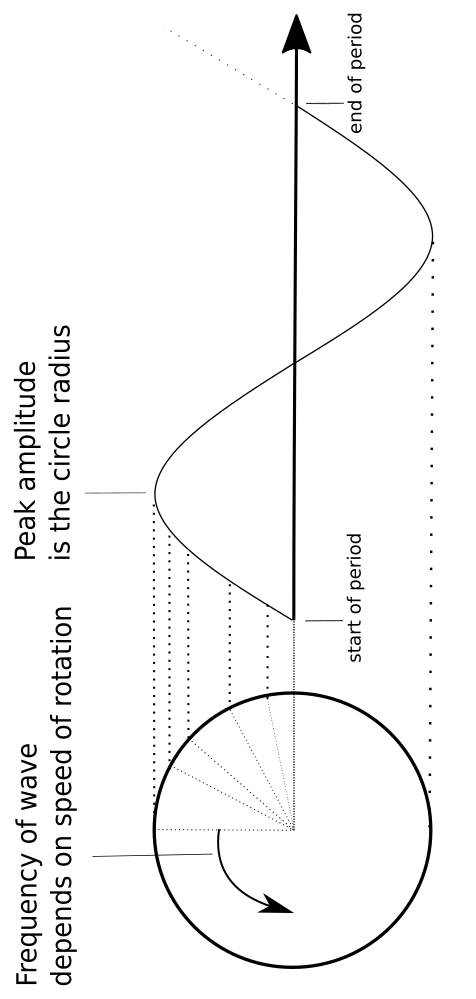
\includegraphics[width=0.45\linewidth,angle =-90 ]{images/periodic_function.png}
\caption{A computer can simulate waveforms by utilizing periodic functions. Digital waveforms are discrete approximations of analogue waves. Figure adapted from Mitchell~\cite{mitchell2009basicsynthChap5} }
\end{figure*}


 Most organic sounds---sounds from the natural environment, and its flora and fauna---are much more complex than the output of a single oscillator. In such cases, their digital approximation requires a combination of multiple (perhaps thousands) of pure tones. However, with careful programming, DSP techniques can be used to replicate almost any sound, which is why they have driven commercial digital synthesizers for over half a century \cite{jenkins2019analog} and continue to remain a popular method of audio synthesis among artists. Another advantage to using DSP for sound generation is that the synthesizers we build using these functions are tractable: the output is reproducible given the same parameters. This makes the evaluation of a set of inputs (or parameters) to our synthesizers simpler compared to the evaluation of synthesizers that utilize probabilistic models.
 
In the next chapters we will discuss our work towards a system for automatic \textit{generation of sounds}, capable of rapid generation of short (under 1 second) audio clips. Our approach entailed the implementation of a virtual sound synthesizer that can take a set of instructions, or \textit{programs}, as input and generate the corresponding audio. A by-product of this approach is that the sounds generated may sound extremely in-organic, yet perfectly usable by more experimental artists, adding a desirable "novel" factor. 



\subsection{How Can a Computer Evaluate Sounds?}
Automatic evaluation of sounds is an essential component of our work: A thorough manual evaluation of outputs is not possible when hundreds can be created in a second. How can a computer help us evaluate sounds?

Suppose a person is given a set of recordings of solo musical instruments being played by various skill levels and asked to categorize them however they please. There is a long list of features that the person could use for unsupervised categorization: the length of audio recordings, the skill of the player, timbre, rhythm, and so on. 

Sounds can be represented digitally as a series of numbers (discussed further in Section~\ref{sec_sampling_rates}). Given this representation, computers can be programmed to quickly extract the majority of these feature types for us. With shorter audio clips (such as the drum sounds we're interested in), personal subjectivity might play a smaller role in describing sounds, making the categorization task easier.

In our work, we find simple features such as frequency content (high pitch vs low pitch), length, and envelope (change in loudness, how fast the sounds reaches its maximum loudness and fades away) to be powerful for the categorization of drum sounds. We will discuss our algorithms for extraction of these and other features in Chapter ~\ref{implementation}. We will also discuss how these extracted features were used to train models that can automatically categorize new sounds.  
\section{What Is Our Methodology?}
\label{sec_methodology}
We conceptualized a general pipeline for approximation of sounds: A synthesizer is randomly programmed, while a virtual ear rapidly evaluates assigns a score to the sound outputs, this score is used for the separation of undesired outputs from desired ones. This approach assumes that a fraction of the randomly generated sounds can be substituted for percussion and that the virtual ear will assign higher evaluation scores to this subset. Our implementation allows for the improvement of heuristic search algorithms such that the parameters of the synthesizer can be selected based on the previously observed evaluations. Following this idea, we found the proper implementation of 2 major components to be crucial:

\begin{itemize}
    \item \textit{Virtual Synthesizer}: A flexible, deter\-min\-istic, and tract\-able gener\-ator which can create audio. 
    \item \textit{Virtual Ear}: A classifier that returns an evaluation of an audio sample; estimating the effectiveness of an audio sample's fulfillment of a producers requirements. The ear's evaluation guides the generation process towards a desired path, making it a crucial component of our pipeline. 
\end{itemize}

Our components are designed with modularity and parallelizability in mind. This allows each component to be debugged, modified, and improved without requiring modifications in other components while additionally increasing the scalability and speed of experiments. 
Section~\ref{implementation} contains further discussion of the components as well as the code that glues the project together.

While the main focus of this project is the generation of novel percussive sounds, our methodology indicates promising results with regards to creation of new presets for any virtual synth without the need for a-priori knowledge of the functions or its parameters (i.e the effect of parameter modulation on the sonic output). We also demonstrate the viability of a virtual synthesizers based on Digital Signal Processing (DSP) methods for fast, unsupervised creation of novel audio. 


% Instead of learning weights and parameters in an audio-generation neural network, we wish to generate, search, and tune synthesizers to produce percussion sounds. Discussed in more detail in section \ref{related}. 


\section{Long and Short-Term Goals}
We wish to leverage AI technologies, heuristic search, and DSP methods for the synthesis of novel audio. The work here is motivated by the idea of finding new, convenient methods for the expansion of a music producer's library of sounds. We demonstrate our work in combining machine listening and automatic synthesizer programming to find pieces of audio which can be used as drums. Using the generation of short, percussive audio samples as a starting point, this project is a proof of concept for a modular, generative pipeline of novel, one-shot audio samples. Design decisions were made such that this approach can be modified for creation of other, non-percussive sound-types. 

The goal here is to create an unsupervised system that generates discrete sounds which are suitable substitutes for one-shot recordings of organic drums. In addition, given that a sound is percussive, we require the accurate categorization of drum-types. These definitions can be subjective and/or context dependent: \enquote{suitable substitute} varies by producer and type of music, and we can only define \enquote{one-shot recordings of organic drums} via examples. These definitions necessitate that the results of this system, the agreement between the outputs of the system and individuals needs to be measure in a blinded way. 

% We created systems capable of generating drum synthesizer programs, and measured the success rate by listening to the sound outputs. The survey of our best generative system showed that only 8\% of the sounds were deemed not percussive by both reviewers, and 30\% by at least one. With regards to agreement between manual and automatically assigned labels, our measurements showed Fleiss kappa scores of 0.35 or higher, indicating a moderate agreement.

\end{document}